\chapter{Results}
\label{chapter:Results}

\section{Results of simulated tasks}
\label{section:results_metaworld}
\subsection{Performance of task plate\_slide\_v2}
\label{subsection:Performance of task plate_slide_v2}

 \begin{figure}[htpb]
  \centering
  \subfloat{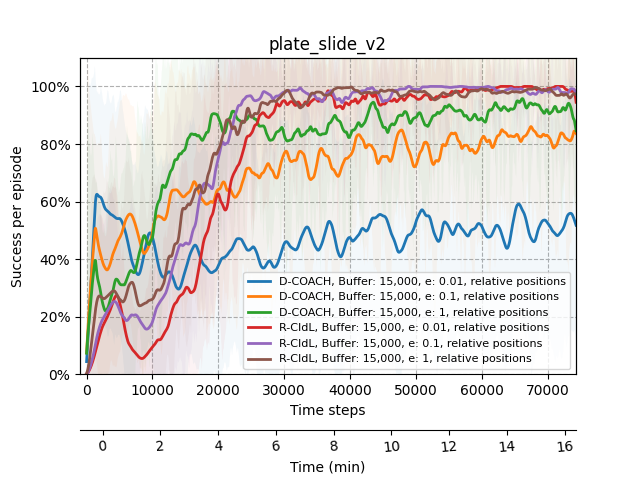
\includegraphics[width=0.5\textwidth]{figures/hockey_same_buffer_V1.png}\label{fig:plate_slide_same_buffer}}
   \hfill
  \subfloat{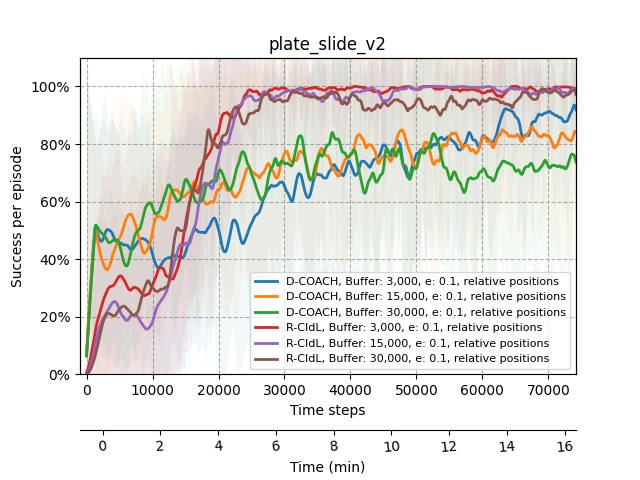
\includegraphics[width=0.5\textwidth]{figures/hockey_same_e_V1.png}\label{fig:plate_slide_same_e}}
  \caption{plate\_slide\_v2 results using a simulated teacher $P_h: \alpha = 0.9; \tau =  0.000015$. On the left, a comparison of the influence of the $e$ parameter on the baseline method D-COACH and on R-CIdL. On the right, a comparison of how different buffer sizes affect both methods.}
  \label{fig:results_plate_slide_buffer_e}
\end{figure}


      
blab bla


\begin{figure}[H]
    \centering
    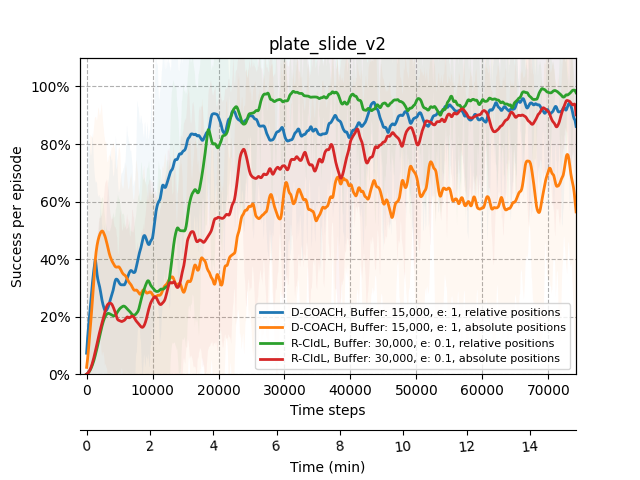
\includegraphics[width=.7\textwidth]{figures/hockey_best_v2.png}
    \caption{plate\_slide\_v2 results using a simulated teacher $P_h: \alpha = 0.9; \tau =  0.000015$. Comparison of the best performance of each method in relative positions, against their performances in absolute positions with the same conditions of buffer and $e$.}
    
    
    \label{fig:results_plate_slide_best}
\end{figure}

\subsection{Performance of task drawer\_open\_v2}
\label{subsection:Performance of task drawer_open_v2}


 \begin{figure}[H]
  \centering
  \subfloat{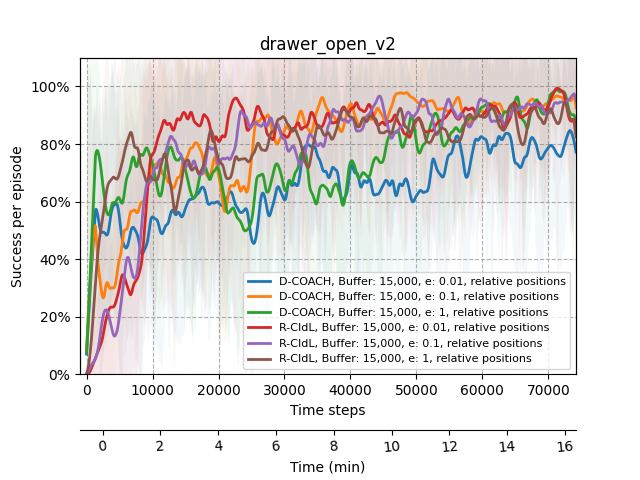
\includegraphics[width=0.5\textwidth]{figures/drawer_same_buffer.png}\label{fig:drawer_open_same_e}}
   \hfill
  \subfloat{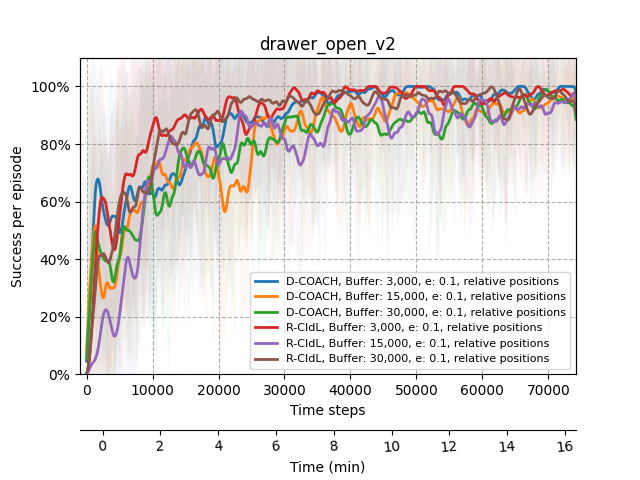
\includegraphics[width=0.5\textwidth]{figures/drawer_same_e.png}\label{fig:drawer_open_same_buffer}}

  \caption{drawer\_open\_v2 results using a simulated teacher $P_h: \alpha = 0.9; \tau =  0.000015$. On the left, a comparison of the influence of the $e$ parameter on the baseline method D-COACH and on R-CIdL. On the right, a comparison of how different buffer sizes affect both methods.}
  \label{fig:results_drawer_open_buffer_e}
\end{figure}

\begin{figure}[H]
    \centering
    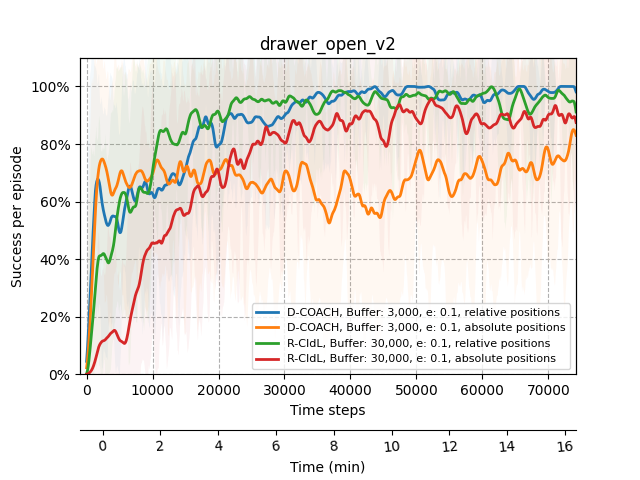
\includegraphics[width=.7\textwidth]{figures/drawer_best.png}
    \caption{drawer\_open\_v2 results using a simulated teacher $P_h: \alpha = 0.9; \tau =  0.000015$. Comparison of the best performance of each method in relative positions, against their performances in absolute positions with the same conditions of buffer and $e$.}
    \label{fig:results_drawer_open_best}
\end{figure}


\section{Results of validation in real system}
\label{section:results_kuka}

To validate the proposed R-CIdL algorithm in a real system, we taught the 2 planar manipulation tasks described in sections \ref{subsection:Park a box} and \ref{subsection:Push box in a straight line}. The human teaching provided the necessary corrections to the position of the end effector via a joystik. In this subsection we show the results obtained for both tasks and because the objective is simply to validate R-CIdL, we did not performed comparisons with other methods. 



 Based on some initial trials, a correction magnitude (i.e. error constant e) of 5 centimeters is found to work well for the task. The minimum height of the end effector is limited such that the ball does not hit the ground plane. For safety reasons, the joint angles are also limited to between zero and 90 degrees. To avoid the ball rolling off the sides of the cup and thus moving

\subsection{Task 1: Push a box}
\label{subsection:results_kuka_push}


165 episodes, evaluation every 5 episodes

7365 feedback signals
Accumulated timesteps 13135
e 0.5, buffer 10000 that never gets fully complete meaning that all the feedback provided is used to update the HumanModel
Average timesteps per episode 72

aprox 20 secs per episode

at episode 60, 23 min the slope of the curve starts increasing until 130 episode (47 min) when the percentage of success is 80% aprox



\begin{figure}[H]
    \centering
    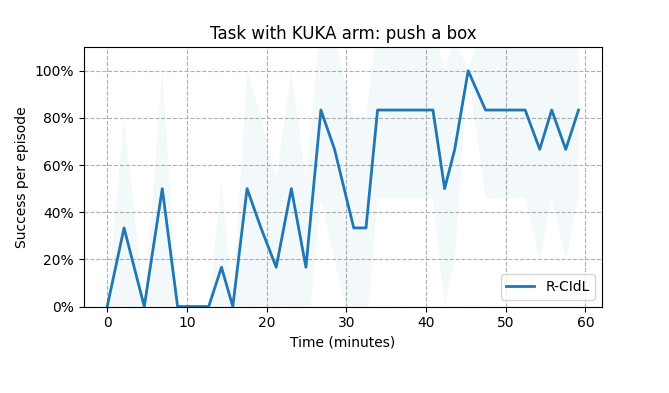
\includegraphics[width=.7\textwidth]{figures/push_1.png}
    \caption{Results of the task "push the box" with a human teacher.}
    \label{fig:kukapush}
\end{figure}

\subsection{Task 1: Park a box}
\label{subsection:results_kuka_park}


From the last episodes of the training, pick the one that seems to show the last best performance, in this case, the episode number 63
3. Perform the evaluations, evaluating every 5 episodes. For this task I did 5 evaluations

At minute 25 the performance increases drastically. This point corresponds with the moment tha the agent learns to go around the corner, Until then all episodes logically fail
At episode 37, the performance has reached its maximum as all the following episodes are succesful.

Here the parameter e was find to work best with a value of 0.3

3390 feedback signals.
every episode on average 36 seconds.
timesteps 12424
\ref{fig:kukapark}


\ref{fig:kukapark}
\begin{figure}[H]
    \centering
    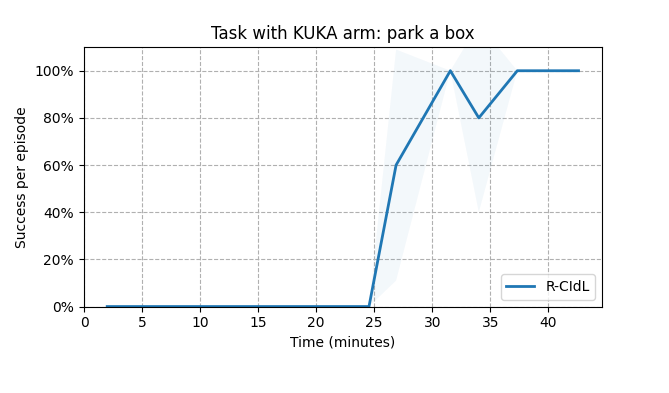
\includegraphics[width=.7\textwidth]{figures/park_1.png}
    \caption{Results of the task "park the box" with a human teacher.}
    \label{fig:kukapark}
\end{figure}